\documentclass[ngerman, a4paper, 11pt]{scrreprt}
\usepackage{lmodern}\usepackage[T1]{fontenc}
\usepackage[latin9]{inputenc}
\usepackage[a4paper,
left=3.5cm, right=3cm,
top=3cm, bottom=3cm]{geometry}
\usepackage{setspace}
\usepackage[multiple]{footmisc}
\geometry{verbose,a4paper}
\setcounter{secnumdepth}{3}
\setcounter{tocdepth}{3}

%%%%%%%%%%%%%%%%%%%%%%%%%%%%%% User specified LaTeX commands.
\usepackage{fancyhdr}
\usepackage{lipsum}
\usepackage{microtype}
\usepackage[clearempty]{titlesec}
\usepackage[ngerman]{babel}

\usepackage{jurabib}
\jurabibsetup{
    commabeforerest,
    ibidem=strict,
    citefull=first,
    see,
    titleformat={colonsep,all},
}
%\usepackage{bibgerm}
\usepackage{array}
\usepackage{pst-pdf}


%for autoref
%There are macros to change the default output with the help of the \renewcommand:
%\figurename             *\figurename*
%\tablename              *\tablename*
%\partname               *\partname*
%\appendixname           *\appendixname*
%\equationname           *\equationname*
%\Itemname               *\Itemname*
%\chaptername            *\chaptername*
%\sectionname            *\sectionname*
%\subsectionname         *\subsesctionname*
%\subsubsectionname      *\subsubsectionname*
%\paragraphname          *\paragraphname*
%\Hfootnotename          *\Hfootnotename*
%\AMSname                *\AMSname*
%\theoremname            *\theoremname*

\usepackage[german]{algorithm2e}
\usepackage{yhmath}
\usepackage{amsmath}
\usepackage{graphicx}
\usepackage{subfig}

\usepackage{blindtext}
\usepackage[colorlinks=false, pdfborder={0 0 0}]{hyperref}

%%\input{german-backcitecom}

%%%% format
\setlength{\parindent}{3em}
\setlength{\parskip}{\baselineskip}
% \onehalfspacing

%% Definitions
\newcommand{\projname}{OGL-Haskell}
\newcommand{\titel}{Modern OpenGL Engine in Haskell}
\newcommand{\untertitel}{Funktionale Konzepte und Implementierung}
\newcommand{\authorname}{Jan-Philip Loos}
\newcommand{\thesisname}{Master Thesis}
\newcommand{\institute}{Fachhochschule Wedel}
\newcommand{\Datum}{01. Mai, 2015}
\newcommand{\warn}[1]{\textcolor{orange}{#1}}
\DeclareMathAlphabet\mathbfcal{OMS}{cmsy}{b}{n}
\defbibheading{head}{\chapter{Literaturverzeichnis}}


\ifpdf
  \usepackage{hyperref}
  \definecolor{darkblue}{rgb}{0,0,.5}
  \hypersetup
    { colorlinks=true
    , breaklinks=true
    , linkcolor=darkblue
    , menucolor=darkblue
    , urlcolor=darkblue
    , pdftitle={\projname -- \untertitel}
    , pdfsubject={\thesisname}
    , pdfauthor={\authorname}
    }
\else
\fi

%% Listings %%%%%%%%%%%%%%%%%%%%%%%%%%%%%%%%%%%%%%%%%%%%%%%%%%%%%%%%%
\usepackage{listings}
\KOMAoptions{listof=totoc} % necessary because of scrhack
\renewcommand{\lstlistlistingname}{Quelltextverzeichnis}
\lstset
  { basicstyle=\small\ttfamily
  , breaklines=true
  , captionpos=b
  , showstringspaces=false
  , keywordstyle={}
  }

\lstnewenvironment{inlinehaskell}
{\spacing{1}\lstset{language=haskell,nolol,aboveskip=\bigskipamount}}
{\endspacing}

\lstnewenvironment{inlinexml}
{\spacing{1}\lstset{language=XML,nolol,aboveskip=\bigskipamount}}
{\endspacing}

\newcommand{\haskellinput}[2][]{
  \begin{spacing}{1}
  \lstinputlisting[language=Haskell,nolol,aboveskip=\bigskipamount,#1]{#2}
  \end{spacing}
}

\newcommand{\haskellcode}[2][]{\mylisting[#1,language=Haskell]{#2}}

\newcommand{\mylisting}[2][]{
\begin{spacing}{1}
\lstinputlisting[frame=lines,aboveskip=2\bigskipamount,#1]{#2}
\end{spacing}
}


\addbibresource{bib/haskell-engine.bib} 

\begin{document}
\pagenumbering{roman}

% \pagestyle{plain}
\pagestyle{scrheadings}
% \pagestyle{fancy}


%%%%%%%%%%%%%%%%%%%%%%%%%%%%%% Titlepage
\titlehead{
  \centering
  \includegraphics[width=.5\textwidth]{img/fhw}\\
  \bigskip
  \textsc{\Large Fachbereich Informatik}
}

\subject{\thesisname}
\title{\titel}
\subtitle{\Large \untertitel}
\date{\vspace{-1cm}{\small Eingereicht:}\\\medskip\Datum}
\author{}
\publishers{\vfill
  \normalsize
  \begin{minipage}{13cm}
  
    \raggedright
    {\small Eingereicht von:} \\
    \smallskip
    {\Large \authorname\ (Mat.-Nr.: 9912)}\\
     Kielmannseggstra{\ss}e 65\\
     22043 Hamburg\\
     Tel.: (+49)~160~966\,511\,88\\
     E-mail: jloos@maxdaten.io\\
     \medskip
     Fachsemester: \warn{XX}\\
     Semester: \warn{XX}\\

    
    \bigskip
    \bigskip
       
    \begin{multicols}{2}
      \raggedright
      {\small Referent:}\\
      \smallskip
      {\Large Prof. Dr. C.-A. Bohn}\\
      Fachhochschule Wedel\\
      Feldstraße 143\\
      22880 Wedel\\
      Phone: 00000000\\
      E-mail: bo@fh-wedel.de\\
         
      \raggedleft
      {\small Korreferent:}\\
      \smallskip
      {\Large Prof. Dr. Uwe Schmidt}\\
      Fachhochschule Wedel\\
      Feldstraße 143\\
      22880 Wedel\\
      Phone: (041\,03)~80\,48-45\\
      E-mail: si@fh-wedel.de\\
    \end{multicols}
 \end{minipage}
}

\maketitle

% our back titlepage
\begin{titlepage}
{
\centering
{\huge \titel}\bigskip\\  
{\Large \untertitel}\bigskip\\
{\large \thesisname\ von\ \authorname}\bigskip\\
}
\paragraph{Abstrakt:}\warn{\blindtext}
\par\vfill
\centering
\footnotesize{
\authorname \bigskip\\
\ccbysa\\
Dieses Werk ist lizenziert unter einer Creative Commons Namensnennung\\
Weitergabe unter gleichen Bedingungen 4.0 International Lizenz.\bigskip\\
Layout done with {\rmfamily \LaTeXe}, {\sffamily \KOMAScript} and {\rmfamily B\textsc{ib}\LaTeX}.
}
\end{titlepage}
\clearpage

\cleardoublepage

%%% blank site
\thispagestyle{empty}
\null\newpage


%%%%%%%%%%%%%%%%%%%%%%%%%%%%%% Table of Content

\thispagestyle{empty}
\tableofcontents
\cleardoublepage

%%% blank site
\thispagestyle{empty}
\null\newpage


\listoffigures
\listoftables
\lstlistoflistings
\chapter{Abkürzungsverzeichnis}
\begin{acronym}
    \acro{GI}{Global Illumination oder Globale Beleuchtung}
    \acro{SVOGI}{Sparse Voxel Octree Global Illumination}
    \acro{SM}{Shadow Map oder Schattentextur}
    \acro{LM}{Lightmap oder Lichttextur}
    \acro{RM}{Radiance Map oder Strahldichtetextur}
    \acro{LPV}{Light Propagation Volume}
    \acro{SSS}{Subsurface Scattering}
    \acro{PBR}{Physically Based Rendering oder Physically Based Shading}
\end{acronym}
\cleardoublepage

\thispagestyle{headings}
\pagenumbering{arabic}


%%%%%%%%%%%%%%%%%%%%%%%%%%%%%% Einführung
\chapter{Einführung}

Diese Einführung dient als Wegweiser durch die vorliegende Arbeit und soll einen kurzen Überblick über die folgenden Kapitel und deren Inhalt geben.

\section{Überblick}

In \fref{chap:engine-uebersicht} wird mit einer Übersicht über die aktuellen Strömungen der Spiele- und Grafik-Engine-Entwicklung begonnen. Das Kapitel wird aufzeigen, dass Spieleengines komplexe, dynamische und interdisziplinäre Softwareprojekte sind. Die unterschiedlichen Engines teilen einige gemeinsame Anforderungen und Herausforderungen. Das Kapitel wird einige der gemeinsamen Herausforderungen aufzeigen, von denen sich viele auch auf Projekte aus anderen Branchen übertragen lassen.

Abseits der Komplexität von Spiele-Engines gibt es seit wenigen Jahren Bestrebungen die bestehenden, über die Jahre gewachsenen, Grafikschnittstellen wie \textit{DirectX} oder \textit{OpenGL} flexibler zu gestalten aber auch in vielen Bereichen deutlich zu verschlanken. Das \fref{chap:modern-opengl} betrachtet diese Entwicklung exemplarisch an \textit{OpenGL}, und konkretisiert den Begriff \textit{Modern OpenGL} mit praktischen Bezügen.

\section{Motivation}

Aus den gewachsenen Anforderungen an komplexe Softwareprojekte wird in \fref{chap:loesungen-durch-fp} die Motivation begründet, nach neuen Hilfmitteln und Konzepten zu suchen, die behilflich sind die Komplexität beherrschbar zu halten und die Anforderungen besser zu erfüllen. Das Kapitel diskutiert anhand von Haskell, ob und wie funktionale Programmierung bei der Erfüllung der Anforderungen hilfreich sein kann.

Viele Neuerungen in den Grafikschnittstellen ermöglichen oder erzwingen neue Denkansätze für die Entwicklung von Grafikanwendungen. \Fref{chap:haskell-modern-gl} zeigt auf, welche Möglichkeiten sich für den Einsatz von Haskell mit den Neuerungen in den Grafikschnittstellen auftun. Anschließend werden aktuelle Grafik-Engines in Haskell diskutiert \warn{konkretisieren was diskutiert wird}.

\section{Ziel}

Der Kern der vorliegenden Arbeit befasst sich damit, eine flexible und komponierbare Grafikpipeline in Haskell zu entwickeln. Aufbauend auf dem Konzept eines Mealy-Automatens wird in \fref{chap:ueberblick-pipeline} die grundlegende Form der Pipeline-Bausteine entwickelt. Anschließend werden einige abstrakte und funktionale Konzepte erläutert und zur Anwendung gebracht. Es wird anhand von kleinen Beispielen demonstriert, wie die funktionalen Konzepte dabei helfen, dass sich die Bausteine leicht komponieren und zu komplexeren Systmen zusammensetzen lassen. Zusätzlich hilft die kurz vorgestellte sogenannte Arrow-Notation (\warn{wo vorgestellt}), komplexe Systeme übersichtlich und verständlich zu halten.

Das Konzept des \acl{PBR} gilt als aktueller Stand der Technik in den Echtzeit Rendering-Verfahren. Es soll die Komposition der Texturen in unterschiedlichen Beleuchtungssituationen vereinfachen und vereinheitlichen. \ac{PBR} wird in theoretischen und praktischen Grundlagen in \fref{chap:pbr} vorgestellt. Unter Verwendung des zuvor entwickelten Pipeline-Konzepts, wird das praktische Ziel dieser Arbeit die Umzusetzung einer \ac{PBR} Pipeline sein.

\section{Ergebnis}
Da die entwickelte \ac{PBR} Pipeline zu umfangreich für eine umfassende Betrachtung im Detail ist, wird in \fref{chap:anwendung} exemplarisch ein Renderschritt der Pipeline als Baustein implementiert. Einen zusätzlichen Überblick über das Gesamtsystem der praktischen Implementierung bietet \fref{lst:src-pipeline} im Appendix. Darüber hinaus ist das Gesamtprojekt zu dieser Arbeit als DVD im Appendix in \fref{chap:dvd} angefügt.

Die entwicklete \ac{PBR}-Pipeline wird in \fref{chap:analyse} sowohl auf ihr Echtzeitverhalten als auch grafische Qualität beurteilt. Zusätzlich werden die produktiven Gesichtspunkte, beispielsweise Flexibilität und Wartbarkeit, untersucht. Probleme und Herausforderungen, die sich während der praktischen Umsetzung aufgetan haben, werden ebenso kurz benannt und eingeordnet.

Abgeschlossen wird der schriftliche Teil der Arbeit in \fref{chap:ausblick} mit einem Überblick über zukünftige Ansätze und Bereiche, in denen die Grafik-Engine sich sinnvoll erweitern oder anwenden ließe.

\warn{Image}

\cleardoublepage

%%%%%%%%%%%%%%%%%%%%%%%%%%%%%% Engines
\chapter{Aktuelle Engineentwicklung}
\label{chap:engine-ueberblick}

Moderne Engines zählen inzwischen zu den komplexesten Softwareprojekten. Die Echtzeitanforderung wird immer eine Herausforderung bleiben, da mit neu verfügbarer Resourcen oder frei werdenen Resourcen die Grenze des machbaren verschoben wird.

Moderne Engines richten sicht nicht mehr zwingend ausschließlich an Programmierer, sondern sind inzwischen zu Tools herangewachsen, die es sogar nicht Programmierern erlauben eigene Programmlogiken zu implementieren.

kolaborative unreal engine 5

tools/engines werden nicht mehr einfach am reißbrett entworfen sondern die entwicklung muss dynamisch auf die anforderungen reagieren.
entwicklung niemals abgeschlossen. 
%% Zitat: "Even if the software was perfect when you ship it, it has to adjust, because the world around is changing"

\cleardoublepage

%%%%%%%%%%%%%%%%%%%%%%%%%%%%%% Überblick Modern OpenGL (4.0+)
\chapter{Überblick über Modern OpenGL 4.0+}
\label{cha:modern-opengl}

\cite{gamedevnet:glnext}

\cleardoublepage

%%%%%%%%%%%%%%%%%%%%%%%%%%%%%% Funktionale Progammierung & Modern GL
\chapter{Funktionale Programmierung \& OpenGL}
\label{chap:haskell-modern-gl}

Funktionale Programmierung beschreibtich

\ac{DSA} und die verstärkte Verwendung von Buffern für Daten und Kommands (indirectes Rendering) eröffnet neue Spielräume. Währned häufige Foreign Calls in Haskell zu eigenen Bottlenecks führen können (\warn{Beleg}), helfen die Konzepte generell den CPU Overhead zu reduzieren. Während der CPU Overhead im generellen reduziert wird, reduziert sich zusätzlich der Overhead durch die Reduzierung der Foreign Calls. Der gewonnene Spielraum kann für mehr CPU basierte Aufgaben verwendet werden, aber auch um wartungsunfreundliche Kompromisse zwischen Performance und Code-Hygene. Viele Portierungen von Konsole zu PC erwiesen sich oft als zusätzlich aufwändig, da spezielle Optimierungen auf einzelne Anwendungen die Wartung entsprechender Abschnitte deutlich erschwerten (\warn{BELEG}).

- Spielräume
- Kapselung (Uniform StateVars Quine) Koposition (Applikative, Functoren)

\cleardoublepage

%%%%%%%%%%%%%%%%%%%%%%%%%%%%%% Entwicklung einer Grafikengine in Haskell
\chapter{Überblick über den Kern der Engine}
\label{chap:ueberblick-pipeline}

Auf Grund des Umfangs des Projekts ist es nicht möglich einen all umfassenden Überblick über die Engine zu geben. Die Betrachtung im Detail beschränk sich im Folgenden auf die entwickelte Renderkomponente der Engine und die dahinter stehenden Konzepte und Überlegungen.

\section{Das Rendersystem}

% anforderung
Moderne Renderverfahren (wie zum Beispiel \warn{Deferred Rendering}) bestehen aus mehreren einzelnen Renderschritten. In der Regel erzeugt jeder Renderschritt Daten, oft in Form von Texturen oder Buffern, die dann im fortlaufenden Verfahren als Basis für weitere Renderschritte dienen.
% Netzwerk

% Ziel
% - äußere logik komponierbar / flexibilät
% - vermeidung von Implementierungdetails in der äußeren logik
% - implementierungen nah an opengl (verzicht auf abstraktionsschicht)

Die Konzeption des Rendersystem wurde mit dem Ziel verfolgt die einzelnen Renderschritte eines modernen verzögerten Rendersystems 

\subsection{Mealy als formale Basis}

Das Rendersystem basiert auf dem Konzept eines Mealy Automatens \parencite{Mealy1955}. Ein Mealy Automat ist \ac{FST}, ein spezieller endlicher Automat, der nicht nur seine Eingabesprache vom Eingabeband akzeptiert sondern auch eine Ausgabe auf einem Ausgabeband erzeugt. Ein Transduktor übersetzt die Eingabesprache in eine Ausgabesprache. Bei dem Mealy Automaten als spezielle Form eines \ac{FST} definiert sich die Ausgabe über den momentanen Zustand und die Eingabe auf diesem Zustand. Formal lässt sich ein Mealy Automat $\mathbfcal{M}$ als 6-Tupel wie folgt definieren:

\begin{align}
\mathbfcal{M} = \left( Q, \Sigma, \Omega, \delta, \lambda, q_0 \right)
\label{def:mealy-formal}
\end{align}
\begin{align*}
	\text{mit}\\
	Q &: \text{Endliche Menge von Zuständen} \\
	\Sigma  &:\text{Endliches Eingabealphabet} \\
	\Omega  &:\text{Endliches Ausgabealphabet} \\
	\delta  &:\text{Zustandsübergangsfunktion}\ Q \times \Sigma \rightarrow Q \\
	\lambda &:\text{Ausgabefunktion}\ Q \times \Sigma \rightarrow \Omega \\
	q_0 &: \text{Startzustand}
\end{align*}

Die Definition ließe sich noch um die Menge der finalen Endzustände $F \subseteq Q$ hin zu einem 7-Tupel erweitern. In unserem Konzept verzichten wir auf definierte Endzustände, da wir prinzipiell jede Eingabe akzeptieren. Nicht akzpetierbare Eingaben stellen wir als externe Ausnahmefälle (Exceptions) dar. Ein vereinfachtes Beispiel für eine nicht akzeptierbare Eingabe ist die Eingabe $\bot$, nach der unser gesamtes System in einen undefinierten Zustand $\bot$ wechselt.

\paragraph{Abstrakte Definition in Haskell}
\label{sec:abstrakte-definition-haskell}

Ein Mealy Automat lässt sich in Haskell abstrakt wie in \fref{lst:haskell-mealy} definieren. {\ttfamily a} beschreibt die Eingabe als Äquivalent zum Eingabealphabet $\Sigma$ der formalen Definition und analog beschreibt |b| die Ausgabe als Äquivalent zum Ausgabealphabet $\Omega$. Die Zustandsübergangsfunktion $\delta$ und die Ausgabefunktion $\lambda$ ergibt sich aus der jeweils konkreten Implementierung des Mealy. Die Menge der Zustände $Q$ wird jeweils von der konkreten Mealy Implementierung gekapselt wie in \fref{lst:state-mealy-beispiel} anhand eines Beispiels veranschaulicht. Aber es lässt sich bereits feststellen, dass die gewählte Form des Mealy Automatens weit mehr als nur ein endlicher Automat ist, da die Mächtigkeit des Ein- und Ausgabealphabets unendlich sein kann, wie dies zum Beispiel bei der Menge der natürlichen Zahlen (abzählbar unendlich) der Fall ist. Daraus folgt zusätzlich, dass auch die Menge der Zustände unendlich sein kann (Zählmaschine).

\begin{haskell}[label={lst:haskell-mealy},caption={[Definition Mealy in Haskell]Definition Mealy in Haskell\protect\footnotemark}]
newtype Mealy a b = Mealy { runMealy :: a -> (b, Maely a b) }
\end{haskell}
\footnotetext{https://hackage.haskell.org/package/machines-0.4.1/docs/Data-Machine-Mealy.html}

Für diese Definition einer Meleay lassen sich einige nützlicher Klassen finden, die wir aber hier überspringen da wir in \fref{sec:konkret-rendersystem} für unsere erweiterte monadische Definition eigene Implementierungen entwickeln werden.

Allgemein lässt sich die Funktionsweise von |Mealy| wie folgt beschreiben: Zu jeder Eingabe |a| erzeugt die Ausfühung von |Mealy| durch |runMealy| eine Ausgabe |b| und einen neuen Mealy-Automaten, der die selbe Eingabesprache in die selbe Ausgabesprache übersetzt. Im einfachsten Fall ist der neu erzeugte Mealy-Automat exakt der gleiche aus dem vorherigen Schritt. Ist dies für das gesamte Eingabealphabet gegeben gilt der Automat als zustandslos.

Für die Konstruktion eines Mealy-Automatens mit lokalem Zustand folgt aus der formalen Definition \ref{def:mealy-formal} die Notwendigkeit einer Zustandsübergangsfunktion $\delta$ und einem Startzustand $q_0$. Hiefür definieren wir uns in \fref{lst:state-mealy-ctr} die Hilfsfunktion |localStateMealy|. Der erste Parameter |s -> a -> (b, s)| beschreibt die Kombination der beiden Funktionen $\delta$ und $\lambda$, der zweite Parameter den Startzustand $q_0$.

\begin{haskell}[label={lst:state-mealy-ctr},caption={[Konstruktion Mealy mit lokalem Zustand]Hilfsfunktion zur Konstruktion eines Mealy-Automatens mit lokalem Zustand}]
localStateMealy :: (s -> a -> (b, s)) -> s -> Mealy a b
localStateMealy stateTransition initState = run initState where
  run state = Mealy (\input -> 
    let (output, state') = stateTransition state input 
    in (output, stateTransition state'))
\end{haskell}

Mit Hilfe der Funktion |localStateMealy| wird ein Mealy-Automat erzeugt, der bei jeder Ausführung die |stateTransition| Funktion auf die aktuellen Eingabe |input| und den momentanen Zustand |state| anwendet um eine Ausgabe |output| und einen neuen Zustand |state'| zu erzeugen. |output| wird in Verbindung mit dem für die nächste Ausführung neu konstruiertem Meleay-Automaten als Resultat zurück geliefert.

In \fref{lst:state-mealy-beispiel} konstruieren wir einen einfachen Mealy-Automaten der ganzzahlige Eingaben akkumuliert und ausgibt. Abschließend wird in \fref{lst:state-mealy-ausfuehrung} ein Ausführungsbeispiel für |sumMealy| demonstriert.

\begin{haskell}[label={lst:state-mealy-beispiel},caption={[Beispiel Mealy-Automat mit lokalem Zustand]Beispiel Mealy-Automat mit lokalem Zustand}]
sumMealy :: Mealy Int Int
sumMealy = localStateMealy sumInState 0 where
	sumInState state input = (state, state + input)
\end{haskell}

\begin{haskell}[label={lst:state-mealy-ausfuehrung},nolol,caption={Ausführung Mealy-Automat mit lokalem Zustand}]
> let m0 = sumMealy
> let m1 = runMealy m 5
> fst m1
0
> let m2 = runMealy m1 8
> fst m2
5
> let m3 = runMealy m2 0
> fst m3
13
\end{haskell}

\subsection{Konkrete Definition des Rendersystems}
\label{sec:konkret-rendersystem}

\subsubsection{Anforderung}
Ein konkretes Rendersystem soll sich aus mehreren \warn{isolierten} Renderschritten, den Renderpasses, zusammensetzen. Durch die rekursive Definition kann ein Renderpass wiederum ein beliebig komplexes Rendersystem darstellen, so dass zwischen Rendersystem und Renderpass nur semantisch unterschieden wird. Jeder konkrete Pass soll einen konkret definierten Eingabetypen und einen konkret definierten Ausgabetypen besitzen. Ein Renderpass übersetzt die Eingabe in eine Ausgabe und kapselt alle dafür notwendigen Zustände und Vorgänge. Zustandsveränderungen sollen nicht direkt von außen vorgenommen werden können. Zu dem internen Zustand eines Renderpasses können unter anderem benötigte Ressourcen wie Framebuffer oder Shader gehören. Der interne Zustand soll nur vom Renderpass selbst sichbar gemacht werden können, und dass auch nur, wenn (ein Teil-) Zustand vom Renderpass in die Ausgabe geleitet wird. Direkte Veränderungen des internen Zustands sind so von vornherein ausgeschlossen, da in Haskell Daten unveränderlich sind \footnote{ausgenommen über Konstrukte wie MVars oder IORefs}.

Die Definition des Mealy-Typens aus \fref{lst:haskell-mealy} dient als gedankliche Grundlage für die folgende Definition des Rendersystem, da wir mit \ref{lst:state-mealy-ctr} gezeigt haben, wie sich Zustände kapseln lassen. Aus den Anforderungen an das Rendersystem OpenGL-Methoden aufzurufen zu können ergibt sich, dass wir das Konzept des Mealy-Typen noch um einen monadischen Basistypen erweitern müssen, damit wir beispielsweise Operationen in der |IO| Monade ausführen können. Damit wir uns auf keinen konkreten monadischen Typen festlegen müssen, konstruieren wir unser Rendersystem als einen monadischen Transformator (Monad-Transformer). Die Form des monadischen Transformators erlaubt es Operationen aus einer anderen Monade, der Basismonade, in unsere Ausführung zu heben (lift). So können wir unserem Rendersystem zum Beispiel über eine |Writer|-Monade die Fähigkeit verleihen Vorgänge zu protokollieren oder über deine |Reader|-Monade können sich die Renderschritte eine unveränderliche Umgebung (Environment) teilen. Durch das sogenannte Stacken von Monaden ist es möglich die Eigenschaften der unterschiedlichsten Monaden unter einer Monade zusammenzufassen, es entsteht ein Monad-Stack.

\subsubsection{Definition}

Aus den oben gegebenen Anforderungen kann jetzt die Definition für |RenderSystem| in \fref{lst:definition-rendersystem} formuliert werden. |m| entspricht der Basismonade, |i| ist der Typparameter für die Eingabe in das Rendersystem und respektive |o| der Typparameter für die Ausgabe. Das Ausführen eines |RenderSystems| liefert, im Gegensatz zum Mealy-Automaten, als Ergebnis eine monadische Operation mit der Ausgabe |o| und dem neuen |RenderSystem| für die nächste Ausführung. In \fref{lst:rendersystem-beispiel-reader} wird ein einfaches zustandsloses |RenderSystem| auf Basis der |Reader|-Monade definiert und in \fref{lst:rendersystem-ausfuehrung-beispiel} exemplarisch ausgeführt. Das |RenderSystem| gibt den momentanen Integerwert der Umgebung auf stdout aus und liefert den Eingabewert unverändert zurück. Der Integerwert der Reader-Monade könnte zum Beispiel einen globalen Frame-Counter repräsentieren.

\begin{haskell}[label={lst:definition-rendersystem},caption={Definition Rendersystem}]
newtype RenderSystem m i o = RenderSystem { runRenderSystem :: i -> m (o, RenderSystem m i o) }
type RenderPass = RenderSystem -- nur ein semantischer Alias
\end{haskell}

\begin{haskell}[label={lst:rendersystem-beispiel-reader},caption={Beispiel Rendersystem mit ReaderT IO als Basismonade}]
type PrintPass = RenderPass (ReaderT IO Int) a a
printFrame :: PrintPass a a
printFrame = RenderSystem (\i -> do
	env <- ask 
	print (show ask)
	return (i,printFrame))
\end{haskell}

\begin{haskell}[label={lst:rendersystem-ausfuehrung-beispiel},caption={Ausführungsbeispiel Rendersystem}]
> let r0 = runReaderT (runRenderSystem printFrame "Hallo") 0
> fst r0
0
"Hallo"
> let r1 = runReaderT (runRenderSystem r0 "Welt!") 1
> fst r1
1
"Welt"
\end{haskell}

Da wir in der praxis unterschiedliche Formen von |RenderPass|es konstruieren werden, definieren wir uns in \fref{lst:renderpass-ctr} Hilffunktionen für die Konstruktion der drei wesentlichen Ausprägungen: 1. zustandslos und unveränderlich, 2. zustandsbehaftet unveränderlich und 3. voll dynamisch.

\begin{haskell}[label={lst:renderpass-ctr},caption={Konstruktoren für einen RenderPass}]
-- 1. zustandslos und unveraenderlich
mkStaticRenderPass :: Monad m => (i -> m o) -> RenderPass m i o
mkStaticRenderPass f = r where r = RenderSystem (liftM (,r) . f)

-- 2. zustandsbehaftet und unveraenderlich
mkStatefulRenderPass :: Monad m => (s -> i -> m (o,s)) -> s -> RenderPass m i o
mkStatefulRenderPass f = go where
  go s = RenderSystem (\i -> do
    (o, t) <- f s i
    return (o, go t))

-- 3. voll dynamisch
mkDynamicRenderPass :: (i -> m (o, RenderPass m i o)) -> RenderPass m i o
mkDynamicRenderPass = RenderSystem
\end{haskell}


%%%
% Klassen
%%%

\subsubsection{Klassen-Instanzen}
\label{sec:rendersystem-klassen-instanzen}

In \fref{sec:abstrakte-definition-haskell} wurde bereits erwähnt, dass sich für den Mealy-Typen nützliche Klassen-Instanzen implementieren lassen. Die konkreten Implementierungen für den Mealy-Typen wurden übersprungen aber wir werden in diesem Kapitel wesentlichen äquivalente Implementierungen für unseren Typen |RenderSystem| entwickeln. Aus Platzgründen werden nur die jeweils minimal notwendigen Definitionen angegeben, vollständige Definition finden sich im Modul |RenderSystem|. Praktische Anwendungen werden mit unter in \fref{chap:anwendungsbeispiele} gegeben, doch kann auch hier aus Platzgründen keine umfassende Übersicht gegegeben werden. Umfassende Beispiele finden sich ebenso im Projekt beispielsweise im Modul |Yage.Rendering.Pipeline.Deferred|.


%%%
% Functor
%%%

\paragraph{Functor} 
Funktoren, im Folgenden Functor genannt, beschreiben in der Kategorientheorie eine strukturerhaltene Abbildung (Homomorphismus) zwischen zwei Kategorien. In Haskell ist die Klasse der Functoren wie in \fref{lst:class-functor} definiert. Das erste intuitive Verständnis eines |Functor|s in Haskell ist eine Containerstruktur deren Inhalt von einem Typen |a| auf den Typen |b| überführt werden kann, ähnlich dem |map| für die Listen. Zur Klasse der Functoren gehören darüber hinaus noch weit mehr Strukturen. Zum Beispiel lassen sich auch die Ergebnisse von Funktionen homomorph in eine andere Kategorie überführen ohne die Struktur der Berechnung zu verändern.

\begin{haskell}[label={lst:class-functor},caption={Functor Klasse\protect\footnotemark},nolol]
class Functor f where
  fmap :: (a -> b) -> f a -> f b 
\end{haskell}
\footnotetext{http://hackage.haskell.org/package/base-4.7.0.2/docs/Data-Functor.html}

\Fref{lst:rendersystem-functor} definiert eine Functor Instanz für den |RenderSystem| Typen. Beschrieben wird die Überführung des Ergebnistypens |o| in einen neuen Ergebnistypen |c| (siehe konkrete Signatur für |fmap|). Die Implementierung verdeutlich, dass die Struktur der Berechnung nicht verändert wird. Es wird lediglich der Ausgabetyp des |RenderSystem| in einen neuen Ausgabetyp überführt. Diese Functor Instanz ermöglicht es beispielsweise den Ausgabetypen eines |RenderPass|es, mit Hilfe einer Tranformationsfunktion |f| als Adapter, auf den Eingabetypen eines nachfolgenden |RenderPass| zu überführen.

\begin{haskell}[label={lst:rendersystem-functor},caption={Functor Instanz für RenderSystem}]
instance Monad m => Functor (RenderSystem m i) where
  fmap :: (o -> c) -> RenderSystem m i o -> RenderSystem m i c
  fmap f (RenderSystem sys) = RenderSystem (sys >=> \ (o,sys') -> return (f o, fmap f sys'))
\end{haskell}


%%%
% Applicative
%%%

\paragraph{Applicative}
Applikative, im Folgenden Applicatives, sind eine spezielle Ausprägung von Functoren. Ein Applicative wird über zwei Operationen definiert: |pure| bettet einen Wert in den Kontext |f| ein und der Sequenz-Operator |(<*>)| wendet eine Berechnung im Kontext |f| auf einen Wert in |f| an und kombiniert das Resultat \parencite[Kapitel~2]{Paterson2008}. Applicative sind weniger mächtig als Monaden, da sie nur das Sequenzieren von kontextfreien Operationen erlauben. Sie werden gerne dazu verwendet kleine Bausteine als Kombinatoren zu bauen um sie kontextfrei aufeinander anzuwenden. In Haskell sind Applicatives wie in \fref{lst:class-functor} definiert.

\begin{haskell}[label={lst:class-functor},caption={Applicative Klasse\protect\footnotemark},nolol]
class Functor f => Applicative f where
  pure :: a -> f a
  (<*>) :: f (a -> b) -> f a -> f a
\end{haskell}
\footnotetext{http://hackage.haskell.org/package/base-4.7.0.2/docs/Control-Applicative.html}

Für unser |RenderSystem| definieren wir in \fref{lst:rendersystem-applicative} die Applicative Instanz. Auch hier wird anhand der Implementierung von |(<*>)| deutlich, dass die in |sysf| eingebettete Funktion auf den in |sysa| eingebetteten Wert ohne Berücksichtung des Kontext angewendet wird. |pure| entspricht einem RenderSystem, dass ungeachtet der Eingabe konstant den Wert |b| zurück liefert und unter keinen Umständen das Verhalten wechselt. Mit Hilfe der Appliacative Instanz des |RenderSystem|-Typens können wir mehrere Rendersysteme zu einer größeren Struktur kombinieren, sofern die Rendersysteme nicht von einander direkt abhängen. \Fref{lst:rendersystem-applicative-beispiel} zeigt an einem Beispiel, wie über die Applicative Instanz eine Definition eines RenderSystems . Dieses RenderSystem |sceneToTexture| lässt sich dann über die die Applicative Kombinatoren zu einem RenderSystem kombinieren, dass eine Szene in eine Cubemap rendert. Dynamisch erzeugte Cubemaps werden oft als Environment-Maps (Umgebungstexturen) verwendet, um dynamische Spiegelungen der Umgebung auf Objekten darzustellen.

\begin{haskell}[label={lst:rendersystem-applicative},caption={Applicative Instanz für RenderSystem}]
instance Monad m => Applicative (RenderSystem m i) where
  pure b = r where r = RenderSystem (return . const (b,r))
  RenderSystem sysf <*> RenderSystem sysa = RenderSystem (\i -> do
    (f, mf) <- sysf i
    (a, ma) <- sysa i
    return (f a, mf <*> ma))
\end{haskell}

\begin{haskell}[label={lst:rendersystem-applicative-beispiel},caption={Applicative RenderSystem Beispiel}]
data Cube a = CubeTexture{left,right,top,bottom,front,back :: a}

sceneToTexture :: Camera -> RenderPass IO Scene Texture
sceneToTexture = ...

scene :: Scene
scene = ...

-- Cube with cameras along the +/- world axis directions
cubeViews :: Cube Camera
cubeViews = ...

-- Renders a scene into a cube map
sceneToCubeTexture :: RenderPass IO Scene (Cube Texture)
sceneToCubeTexture = Cube
	`fmap` sceneToTexture (left cubeViews)
	<*> sceneToTexture (right  cubeViews)
	<*> sceneToTexture (top    cubeViews)
	<*> sceneToTexture (bottom cubeViews)
	<*> sceneToTexture (front  cubeViews)
	<*> sceneToTexture (back   cubeViews)
\end{haskell}


%%%
% Profunctor
%%%

\paragraph{Profunctor}
Während die vorhergehenden Klassen nur Operationen auf dem letzten Argument des Typens definierten, gehört unser unser |RenderSystem| Typ auch noch weiteren Klassen an, die sich für die letzten beiden Argumente definieren lassen. Ein Functor in zwei Argumenten wird auch Bifunctor genannt. Jedes Argument gehört einer eigenen Functor-Kategorie an, die auch voneinander unterschiedlich sein können aber nicht müssen. Zusammmen bilden die beiden Functor-Kategorien ($C$ und $D$) eine Produktkategorie ($C \times D$) \parencite{MacLane1998}. Ein spezieller Bifunctor ist der Profunctor, dessen erstes Argument contravariant und zweites Argument covariant ist. Ein covarianter Functor entspricht der üblichen Haskell |Functor| Klasse mit einem Morphismus von der Ausgangskategorie hin zur Zielkategorie. Die Contravarianz entspricht dahingehend einem umgekehrten Morphismus, von der Zielkategorie zur Ausgangskategorie. Die Haskell Definition der Klasse |Profunctor| findet sich in \fref{lst:class-profunctor}

\begin{haskell}[label={lst:class-profunctor},caption={Profunctor Klasse\protect\footnotemark},nolol]
class Profunctor p where
  dimap :: (a -> b) -> (c -> d) -> p b c -> p a d
\end{haskell}
\footnotetext{https://hackage.haskell.org/package/profunctors-3.2/docs/Data-Profunctor.html}

Anschaulicher wird die Funktionsweise eines |Profunctor|s wieder bei der Implementierung der |Profunctor| Instanz für unser |RenderSystem|. Das zweite covariante Argument unseres Bifunctors ist unser Parameter |o| für den Ausgabetypen des |RenderSystems| und wird analog zu der Functor Instanz implementiert, mit |g| als Morphismus. Der neue erste Parameter unseres Bifunctors entspricht dem contravarianten Argument. Der umgekehrte Morphismus |f| wird im Gegenzug auf den Eingabewert angewendet, bevor das entsprechende RenderSystem mit der Eingabe ausgeführt wird. Mit der Profunctor Instanz können wir nicht nur elegant den Ausgabetyp unseres Rendersystems konvertieren, sondern auch auch zu einem allgemein definierten Rendersystem neue Varianten erzeugen die auf unterschiedlichen Eingaben arbeiten, solange wir eine Konvertierungsfunktion für die Eingabe definieren können. Die interne Funktionsweise des Rendersystems bleibt trotz etwaiger Konvertierungen von Ein- und Ausgaben die selbe, es werden lediglich die Schnittstellen einem externen Format angepasst.

\begin{haskell}[label={lst:rendersystem-profunctor},caption={Profunctor Instanz für RenderSystem}]
instance Monad m => Profunctor (RenderSystem m) where
  dimap :: (i -> a) -> (b -> o) -> RenderSystem m a b -> RenderSystem m i o
  dimap f g (RenderSystem sys) = RenderSystem (\i -> do
    (o,sys') <- sys (f i)
    return (g o, dimap f g sys'))
\end{haskell}


%%%
% Category
%%%

\paragraph{Category}

Die |Category| beschreibt die Klasse von Strukturen deren Morphismus sich über beide Argumente komponieren lassen. Die grundlegenste |Category| in Haskell ist die der Funktionen und ihre Komponierbarkeit. Unäre Funktionen |(->)| beschreiben einen Morphismus der das Argument der Funktion einem Funktionswert zuordnet. Unäre Funktionen sind in Haskell analog zur mathematischen Funktionskomposition komponierbar. Dies wird dadurch ausgedrückt, dass unäre Funktionen der |Category| Klasse angehören. In \fref{lst:class-category} wird die Definition der Klasse ausgeschrieben. Sie besteht aus dem Identitätsmorphismus |id| und der rechts zu links Komposition |(.)|.

\begin{haskell}[label={lst:class-category},caption={Category Klasse\protect\footnotemark},nolol]
class Category cat where
  id :: cat a a
  (.) :: cat b c -> cat a b -> cat a c
\end{haskell}
\footnotetext{https://hackage.haskell.org/package/base-4.7.0.2/docs/Control-Category.html}

Auch unser Rendersystem beschreibt einen Morphismus von der Eingabe |i| zur Ausgabe |o|. Folglich gehört auch unser |RenderSystem| Typ der Klasse der Kategorien an. In \fref{lst:rendersystem-category} listet die Implementierng der |Category| Klasse für unser |RenderSystem|. Unser Identitätsmorphismus ist ein Rendersystem, dass die Eingabe unverändert ausgibt. Unsere Komposition ist dadurch implementiert, dass wir zuerst die am weitesten rechts stehende Eingabe |a| in unser rechtes |RenderSystem| eingeben und die entsprechende Ausgabe |b| an das linke |RenderSystem| weiter leiten um die finale Ausgabe |c| zu erhalten. Da die jeweiligen Rendersysteme sich dynamisch verändern können, werden die neu erzeugten RenderSysteme ebenso komponiert (|mbc' . mab'|). 

Die erlaubt es uns auf elegenate Weise unterschiedliche Stufen eines RenderSystems hintereinander zu schalten und zu einem größeren Gesamtsystem zu komponieren. \Fref{lst:rendersystem-komposition-beispiel} zeigt an einem Beispiel, wie sich durch die Komposition zweier unabhängig von einander definierten Textur-Filter ein neuer Filter |bloom| erzeugt werden kann.

\begin{haskell}[label={lst:rendersystem-category},caption={Category Instanz für RenderSystem}]
instance Monad m => Category (RenderSystem m) where
  id = RenderSystem (return . (,id))
  RenderSystem mbc . RenderSystem mab = RenderSystem (\a -> do
    (b, mab') <- mab a
    (c, mbc') <- mbc b
    return (c, mbc' . mab'))
\end{haskell}

\begin{haskell}[label={lst:rendersystem-komposition-beispiel},caption={Beispiel einer Komposition von RenderSystem}]
-- Passes colors with Luma above 'threshold'
lumaFilter :: Float -> RenderSystem IO Texture Texture
lumaFilter treshold = ...

-- Filters 'Texture' with a gaussian-kernel of kernelsize x kernelsize
gaussianFilter :: Int -> RenderSystem IO Texture Texture
gaussianFilter kernelsize = ...

bloom :: RenderSystem IO Texture Texture
bloom = gaussFilter 64 . lumaFilter 0.4
\end{haskell}


%%%
% Semigroup
%%%

\paragraph{Semigroup}

Eine \textit{Semigroup} bzw. eine \textit{Halbgruppe} ist eine algebraische Struktur mit einer assoziativen binären Verknüpfung. Sie gilt als Verallgemeinerung eines Monoiden, für die kein neutrales Element benötigt wird und respektive einer \textit{Group} bzw \textit{Gruppe}, für die kein inverses und kein neutrales Element benötigt wird.

\begin{haskell}[label={lst:class-semigroup},caption={Semigroup Klasse\protect\footnotemark},nolol]
class Semigroup a where
  (<>) :: a -> a -> a -- fuer Monoiden 'mappend'
\end{haskell}
\footnotetext{https://hackage.haskell.org/package/semigroups-0.16.2.2/docs/Data-Semigroup.html}

Die Implementierung in \fref{lst:rendersystem-semigroup} verknüpft die beiden |RenderSystem|e, in dem beide auf der gleichen Eingabe sequenziell ausführt werden. Die Resultate werden abschließend mit |(<>)| verknüpft.

\begin{haskell}[label={lst:rendersystem-semigroup},caption={Semigroup Instanz für RenderSystem}]
instance (Applicative m, Semigroup o) => Semigroup (RenderSystem m i o) where
	sysX <> sysY =  RenderSystem (\i -> liftA2 (<>) (runRenderSystem sysX i) (runRenderSystem sysY i))
\end{haskell}

\Fref{lst:rendersystem-semigroup-beispiel} ist ein Beispiel dafür, wie die Resulate aus mehreren Render-Schritten zu einer größeren assoziative Struktur zusammengefügt werden können. In diesem Fall wird mehrfach |downsample| auf auf einer Textur ausgeführt, um anschließend die herunter gerechneten Texturen zu einer Mipmap-Chain zu kombinieren. 

\begin{haskell}[label={lst:rendersystem-semigroup-beispiel},caption={Beispielanwendung Semigroup für RenderSystem}]
import Data.List.NonEmpty
-- | MipmapChain mit einem Basis Element und einer Liste von Mipmap Stufen
-- Instanz von Semigroup
type MipmapChain = NonEmpty

mkBase :: b -> MipmapChain b
mkBase b = b :| []

downsample :: Int -> RenderSystem IO Texture Texture
downsample factor = ...

generateMipmap :: RenderSystem IO Texture (MipmapChain Texture)
generateMipmap = fmap mkBase id 
	<> fmap mkBase (downsample (2^1)) 
	<> fmap mkBase (downsample (2^2)) 
	<> fmap mkBase (downsample (2^3))
\end{haskell}


%%%
% Arrow
%%%

\paragraph{Arrow}

|Arrows| sind eine weitere abstrakte Darstellungsform von Morphismen. Während |Category| die Komponierbarkeit von Morphismen beschreibt, beschreiben Arrows den Morphismus an sich. In Haskell wird ein Arrow über die Operation |arr| und |first| definiert. Zusätzlich gehört zur Arrow Klasse auch die Kompositionsoperation, welche aber schon durch die Spezialisierung von |Category| definiert ist. |arr| stellt den direkten Bezug zu dem grundlegenden Morphismus der unären Funktionen |(->)| und der Arrow Struktur her und hebt einen einfachen Morphismus in den Kontext des |Arrow|s. |first| ist eine Variante, neben dem gespiegelten |second|, der sogenannten Sideline Operation \parencite[Kapitel 1]{Asada2010}. Über |first| kann ein Morphismus |a b c| auf die erste Komponente des Argumentes angewendet werden, während doe zweite Komponente unverändert durchgereicht wird. Erwähnenswert ist abschließend, dass jeder |Arrow| auch als |Profunctor| dargestellt werden kann \parencite[Kapitel 3]{Asada2010}.

\begin{haskell}[label={lst:class-arrow},caption={Arrow Klasse\protect\footnotemark},nolol]
class Category a => Arrow a where
  arr :: (b -> c) -> a b c
  first :: a b c -> a (b, d) (c, d)
\end{haskell}
\footnotetext{https://hackage.haskell.org/package/base-4.7.0.2/docs/Control-Arrow.html}


\begin{haskell}[label={lst:rendersystem-arrow},caption={Arrow Instanz für RenderSystem}]
instance Monad m => Arrow (RenderSystem m) where
  arr f = RenderSystem (\i -> return (f i, arr f))
  first sys = RenderSystem (\ (b,d) -> do
    (c, sys') <- runRenderSystem sys b
    return ((c,d), first sys'))
\end{haskell}

%%%
% ArrowChoice
%%%

\paragraph{ArrowChoice}

Bevor wir zu einem abschließenden Beispiel für die Anwendung der |Arrow| Implementierung unter Verwendung der Arrow-Notation \footnotemark kommen, werden wir im folgenden noch für unser |RenderSystem| die |ArrowChoice| Klasse implementieren um weitere Möglichkeiten der Arrow Notation nutzen zu können. |Arrow|s die auch |ArrowChoice| implementieren können in der Arrow Notation |if| und |case| Konstrukte als syntaktischen Zucker verwenden. Die Definition der |ArrowChoice| Klasse ist in \fref{lst:class-arrowchoice} angeben. |left| beschreibt dabei eine Operation die eine Operation auf das Argument anwendet, wenn das Argument mit |Left| markiert wurde. Wurde das Argument mit |Right| markiert bleibt es unverändert.

\footnotetext{https://downloads.haskell.org/~ghc/7.8.2/docs/html/users\_guide/arrow-notation.html}

\begin{haskell}[label={lst:class-arrowchoice},caption={ArrowChoice Klasse\protect\footnotemark},nolol]
class Arrow a => ArrowChoice a where
  left :: a b c -> a (Either b d) (Either c d)
\end{haskell}
\footnotetext{https://hackage.haskell.org/package/base-4.7.0.2/docs/Control-Arrow.html\#g:5}

Die Implementierung von |ArrowChoice| für unser |RenderSystem| in \fref{lst:rendersystem-arrowchoice} ist trivial. Wurde die Eingabe mit |Left| markiert, wenden wir unser |RenderSystem| auf die Eingabe an und markieren die Ausgabe wiederum mit |Left|. Mit |Right| markierte Eingaben passieren das RenderSystem unverändert und ohne Seiteneffekte.

\begin{haskell}[label={lst:rendersystem-arrowchoice},caption={ArrowChoice Instanz für RenderSystem}]
instance Monad m => ArrowChoice (RenderSystem m) where
  left sys = RenderSystem (\case
    Left i  -> do
      (b, sys') <- runRenderSystem sys i
      return (Left b, left sys'))
    Right i -> return (Right i, left sys)
\end{haskell}

\cleardoublepage

%%%%%%%%%%%%%%%%%%%%%%%%%%%%%% Entwicklung einer Grafikengine in Haskell
\chapter{Physically Based Rendering}
\label{chap:pbr}

\acl{PBR} beschreibt ein relativ neues Oberflächenmaterial- und Beleuchtungskonzept in der Spieleindustrie. Es basiert auf dem von Disney vorgestelltem Beleuchtungsmodell \parencite{Burley2012} oder \parencite{Gotanda}. Während Disney ein festes Beleuchtungsmodell entwickelte, gibt \ac{PBR} kein festes Regelwerk vor und ist daher vielmehr als ein Paradigma zu verstehen, das erlaubt die Wechselwirkung von Licht, Oberflächen und Betrachter allgemeingültig und möglichst akkurat zu simulieren \parencite[Kapitel 1]{Rousiers2014}. Es führt dabei auch kein weiteres Beleuchtungsmodell ein, sondern lässt sich mit unterschiedlichen Approximationen der BRDF nutzen. Nicht desto trotz bedeutet die Umstellung auf ein \ac{PBR} Verfahren eine komplette Umstellung der Produktions- und Renderpipeline. In diesem Kapitel geben wir einen kurzen Überblick über die Prinzipien von \ac{PBR} und Beweggründe, warum es sich lohnen könnte, dieses Konzept praktisch umzusetzen.

\section{Gründe für \acl{PBR}}
\label{sec:pbr-warum}

Die Fähigkeiten einer Grafikengine werden oft daran beurteilt wie plausibel und realistisch die synthetisierten Bilder wirken. Um entsprechende Bilder in Echtzeit rendern zu können, müssen Kompromisse eingegangen werden. Während offline Renderverfahren mehr Freiheiten haben sich dem Realismus anzunähern, sorgen die Approximationen der Ad-hoc Shading Modelle \parencite{Martinez2010} oft für Probleme.

Der Künstler produziert 3D Modelle oft in einer von der Echtzeitengine isolierten Software Umgebung die ihre eigenen realistischem Beleuchtungsmodell besitzen. In den Ad-Hoc Modellen  gibt in der Regel nur wenige Oberflächenparameter, die zusätzlich in keinem physikalischen Zusammenhang zueinader gesetzt werden. Oft lassen sich die unterschiedlichen Parameter gar nicht direkt in einen physikalen Zusammenhang setzen, da sie überwiegend unabhängig von einander eingeführt wurden. Zum Beispiel wird das Ob und Wie Oberflächen die Umgebung spiegeln oft unabhängig vom sonstigen Lichtreflexionsverhalten (z.B. Spekularer Wert) gesteuert. Dies führt oft zu physikalisch inkorrekten Beleuchtungen. Dies führt zu vielen Spezialfällen und vielen Iterationen auf Künstlerseite, bis das Objekt mit der gewünschten Oberflächenbeleuchtung in der speziellen Szeneneinstellung dargestellt wird. Ändern sich die Beleuchtungsparameter und Szeneneinstellungen sind die mühsam justierten Einstellungen wieder hinfällig. 

Mit \ac{PBR} werden die klassischen Ad-hoc zusammengestellten Beleuchtungsmodelle verworfen, damit Beleuchtungsmodelle entworfen werden können, deren Parameter sich in einem physikalisch sinnvollem Zusammenhang setzen lassen. Nur dadurch lassen sich Spezialfälle vermeiden und es lässt sich eine visuelle Konsistenz herstellen. Visuelle Konsistenz bedeutet in diesem Zusammhang, dass sich einmal konfigurierte Oberflächeneigenschaften in unterschiedlichen Beleuchtungssituationen realistisch plausibel und verhersagbar verhalten. 

Dies wird dadurch erreicht, dass die Eigenschaften der Lichtquellen, die Oberflächeneingenschaften und der Betrachter von einander entkoppelt werden. Ziel ist meist ein einheitliches Beleuchtungsmodell zu entwickeln, das für alle möglichen Szeneneinstellungen geeignet ist und in sich konsistent ist.

\section{Theoretische Grundlagen}
\label{sec:pbr-grundlagen}

Beleuchtungsmodelle werden unter dem Begriff \acf{BRDF} zusammengefasst. Allgemein beschreibt eine \ac{BRDF} das Reflexionsverhalten von Oberflächen. Sie lässt sich aus den zwei getrennten Termen für die diffuse $f_d$ und spekulare Reflexion $f_s$ zusammensetzen \parencite[Kapitel 3.1.2, Seite 7]{Rousiers2014}, so dass sich beide Terme getrennt von einander betrachten lassen. Das ermöglicht für $f_d$ und $f_s$ unterschiedliche unterschiedliche Modelle und spezialisierte Approximationen.

Damit die physikalischen Eigenschaften der Oberflächen möglichst realistisch abgebildet werden können, wird ein geeignetes Beleuchtungsmodell (\acf{BRDF}) als Grundlage für die Lichtberechnung benötigt. Die klassischen Modelle wie Phong oder Blinn-Phong bieten hierbei wenige physikalische Einflussgrößen, und sind deswegen ungeeignet. Bei Phong bzw. Blinn-Phong wird zum Beispiel der spekulare Beitrag von Parametern beeinflusst, die sich weder intutiv greifen noch sich ohne weiteres direkt aus physikalischen Oberflächeneingenschaften ableiten lassen. Im Folgenden betrachten wir das Cook-Torrance Modell als Grundlage für unsere \ac{PBR} Implementierung und verwenden die in \fref{tab:pbr-notation} genannte Notation.

\begin{align}
	\label{eq:brdf-dekonstruiert}
	% \caption{Dekonstruierte BRDF}
	f(\vV,\vL) &= f_d(\vV,\vL) + f_s(\vV,\vL)
\end{align}

\begin{table}
\centering
\begin{tabular}{c l}
\hline
	$\vV$ & Richtungsvektor zum Betrachter \\
	$\vL$ & Richtungsvektor zur Lichtquelle \\
	$\vN$ & Oberflächennormale \\
	$\vH$ & Winkelhalbierende ($\frac{V + L}{\|V + L\|}$) \\
	$\vR$ & Reflexion von $L$ an $N$ \\
	$m$ 	 	& Rauheitswert der Oberfläche (\textit{Roughness}) \\
 	$f$ 		& \textit{BRDF} \\
	$f_d$ 		& Diffuser Term der \textit{BRDF} \\
	$f_s$ 		& Spekularer Term der \textit{BRDF}\\
\hline
\end{tabular}
\caption[Notation \textit{BRDF}]{Notation}
\label{tab:pbr-notation}
\end{table}

\warn{Bild BRDF V, N, L, H, R}

\subsection{Cook-Torrance Modell}

Das Reflexionsverhalten von Oberflächen wird in der Realität wesentlich von der Oberflächenbeschaffenheit des Materials bestimmt. Polierte Oberflächen spiegeln, im Gegensatz zu rauhen Oberflächen, die Umgebung und erhalten Glanzlichter bei direkter Beleuchtung. Irreguläre rauhe Oberflächen streuen das einfallende Licht ungleichmäßig in alle Richtungen.

Ein realistisches Reflexionsmodell muss diese Oberflächenbeschaffenheit berücksichtigen. In Echtzeitverfahren ist es nicht praktikabel die mikroskopischen Unebenheiten, genannt \textit{Microfacetten oder Microfecets} (siehe \fref{fig:microfacet}), exakt zu berechenen. Entsprechend wurden einige approximierende Microfacet Modelle entwickelt, die die Interaktion des Lichts mit den Facetten realistisch abbilden können.

\begin{figure}
	\label{fig:microfacet}
	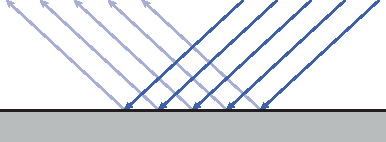
\includegraphics[width=.5\textwidth]{roughness0}
	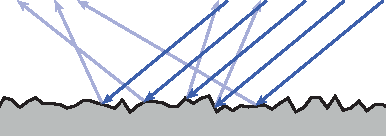
\includegraphics[width=.5\textwidth]{roughness1}
	\caption[Rauheit]{links: $m = 0$; rechts $m = 1$}
\end{figure}

Eines von ihnen ist das Cook-Torrance Modell \parencite{Cook1981}, welches mit dem Ziel entwickelt wurde die physikalischen Reflexionseigenschaften von rauhen und glatten Oberflächen realistischer abzubilden als es die klassischen Modelle ermöglichen \parencite[Seite 40]{Ngan2004}. Da sich das Cook-Torrance Modell auf spekulare Reflexionen konzentriert, verwenden wir das Cook-Torrance Modell auschließlich zur Berechnung des spekularen Anteils $f_s$ der BRDF. Der diffuse Anteil $f_d$ wird durch das klassische Lambert'sche Modell abgebildet und nicht weiter betrachtet. Denkbar sind aber auch andere Modelle für die diffuse Reflexion. In \fref{eq:cook-torrance-model} wird das Modell formal dargestellt.

\begin{align}
	\label{eq:cook-torrance-model}
	% \caption{Cook-Torrance Illumination}
	f_s(\vV,\vL) = \frac{\mathcal{F}(\vV,\vL)D(\vV,\vL)G(\vV,\vL)}{4(\vN \cdot \vV)(\vN \cdot \vL)}
\end{align}

Der spekulare Beitrag $f_s$ wird durch die drei Faktoren bestimmt: Dem Fresnel $\mathcal{F}$ Term, der Microfacet Richtungsverteilung, $D$ und der geometrischen Abschwächung (Geometrical Attenuation) $G$. Die Auswahl der konkreten Approximationen folgt der aus \cite[Seite 3]{Karis2013}.

\subsubsection[Fresnel]{Fresnel $\mathcal{F}$}
Der Fresnel Effekt beschreibt die Beobachtung, dass Oberflächen stärker reflektieren, umso flacher der Betrachtungswinkel wird. Als Approximation wurde die \textit{Schlick Approximation} \parencite{Schlick1994} gewählt. In \cite{Lagarde2012} wurde eine weitere Modifikation vorgeschlagen um den Berechnungsaufwand zu reduzieren. Diese findet hier ebenso ihre Anwendung. $F_0$ beschreibt die Reflektanz für parallel zur Normale $\vN$ einfallendes Licht.

\begin{align}
	\label{eq:fresnel-schlick}
	\mathcal F(\vV,\vL) = F_0  + (1 - F_0) 2^{(-5.55473 (\vV \cdot \vH) - 6.98316 (\vV \cdot \vH))}
\end{align}


\subsubsection[Facetten Normalverteilung]{Facetten Normalverteilung $D$} 
$D$ beschreibt die statistische Normalverteilung der Ausrichtung der Microfacets entsprechend der Winkelhalbierenden $\vH$. Die Microfacets von glatten Oberflächen sind überwiegend gleich ausgerichtet, so dass Licht hauptsächlich entlang $R$ reflektiert wird. Raue Oberflächen besitzen eher zufällig ausgerichtete Mircofacets, so dass das reflektierte Licht breiter gestreut wird. Die Rauheit der Oberfläche wird mit $m$ im Intervall $[0,1]$ ausgedrückt. Zur Approximation von $D$ finden sich wiederum eine vielzahl von Modelle. Die Implementierung verwendet das als \textit{GGX} in \cite{Walter2007} vorgestellte Modell (siehe \fref{eq:ggx}).

\begin{align}
	\label{eq:ggx}
	D(\vV,\vL) = \frac{m^4}{ \pi \left(\left( \vN \cdot \vH \right)^2\left(m^4 - 1\right) + 1\right)^2}
\end{align}


\subsubsection[Geometrische Abschwächung]{Geometrische Abschwächung $G$} 
$G$ beschreibt einen Faktor, der die Tatsache simuliert dass Microfacets sich gegenseitig einfallendes oder reflektiertes Licht blockieren und sich somit gegenseitig schattieren ($G_1(\vL)$) oder Reflexionen maskieren ($G_1(\vV)$) können. Verwendet wird eine modifizierte Version der \textit{Schlick} Approximation, damit sie sich dem physikalisch präziseren Smith Modell annähert. Eine genauere Analyse des Smith Modells findet sich in \cite[Kapitel 6, Seite 33]{Heitz2014}.

\begin{align}
	\label{eq:geometric-schlick}
	k &= \frac{(m + 1)^2}{8}\\
	G_1(\vV) &= \frac{\vN \cdot \vV}{(\vN \cdot \vV)(1-k)+k}\\
	G_1(\vL) &= \frac{\vN \cdot \vL}{(\vN \cdot \vL)(1-k)+k}\\
	G(\vV,\vL) &= G_1(\vV) G_1(\vL)
\end{align}


\subsubsection{Dielektische und metallische Materialien}

\begin{figure}
	\includegraphics[width=.5\textwidth]{dielectric}
	\includegraphics[width=.5\textwidth]{metallic}
	\caption[Dielektische und metallische Materialien]{links: Plastik; rechts: Messing}
	\label{fig:dielectric-metallic}
\end{figure}

In der Natur lassen sich Substanzen bezüglich ihrer Leiteigenschaften in drei Kategorien einteilen: Nichtleiter (Dielektrikum oder Isolatoren), Halbleiter und Leiter (u.A. metallische Substanzen). Ohne auf die physikalischen Details einzugehen (Details in \cite[Abschnitt: Glanz und Farbe der Metalle]{Zawischa2011}) unterscheiden sich metallische und dielektrische Materialien in ihrem spekularem Reflexionsverhalten. Dielektrische Materialien besitzen ausschließlich weiße spekulare Reflexionen\footnote{unter weißem Licht} während metallische Materialien über ein Farbspektrum spekular reflektieren \parencite[Abschnitt: Specular]{Lagarde2011a}(siehe \fref{fig:dielectric-metallic}).

In der Implementierung wird dies über eine Justierung des $F_0$ Wertes aus dem Fresnel-Term $\mathcal{F}$ abgebildet. Für metallische Materialien wird $F_0$ auf die Grundfarbe (Albedo) des Materials gesetzt und die Grundfarbe auf schwarz, ansonsten wird $F_0$ auf weiß gesetzt (Die Idee basiert auf der Unreal Engine 4 Implementierung, Stand 2015).

\section{Praktische Umsetzung}
\label{sec:pbr-umsetzung}


Wie Eingangs erwähnt erfordert die Umstellung auf \ac{PBR} eine Anpassung in der Produktion und der Render"-pipeline. Während Diffuse- bzw. Albeo-Texturen sowie Normalentexturen bereits üblich sind, ist es speziell für die Albedo Texturen wichtig, dass sie von jeglicher vorberechneter Beleuchtung bereinigt sind, damit die grundlegenden Texturen in allen Beleuchtungssituationen anwendbar sind (Details in \cite{Lagarde2011}). Die Implementierung wird im \fref{chap:anwendung} auszugsweise vorgestellt. Im Folgenden eine kurze Übersicht über die praktischen Grundlagen der Implementierung.

\subsection{Eingangsparameter}

Als Eingangsparameter verwendet die Pipeline der Implementierung dieser Arbeit folgende Größen:
\begin{itemize}
\item Albedo-Textur im sRGB Farbraum
\item Normalen-Textur mit Oberflächennormale im Tangenten-Raum kodiert in RGB
\item Roughness-Textur ($m$) in Graustufen
\item Metallic-Textur in Graustufen für die Unterscheidung von dielektrischen und metallischen Oberflächen\footnote{Entspricht einer Maske, 0 = nicht metallisch, 1 = metallisch}
\end{itemize}

\warn{Bild von Beispiel Texturen}

\subsection{Renderverfahren}

Als Renderverfahren wurde das als \textit{Deferred Shading} bekannte Verfahren gewählt, da es effizienter als \textit{Forward Shading} in der Lichtberechnung von vielen Lichtern ist. Dazu wird vor der Berechnung der Schattierung der Oberflächen die Geometrie gerendert. In diesem Renderschritt werden die Oberflächenattribute wie Albedo-Farbe, Roughness und Normale in Texturen gerendert, kombiniert oft \textit{G-Buffer} genannt. Dieser \textit{G-Buffer} dient dann anschließend im Shading Renderschritt als Grundlage für die Berechnung. In diesem Schritt werden die Lichter mit Stellvertreter Geometrien gerendert. Für jedes so erzeugte Fragment wird die gewählte \ac{BRDF} mit Hilfe der Lichtparameter und der Parameter aus dem G-Buffer ausgewertet. In der fortlaufenden Pipeline werden die Farbwerte im HDR-Raum behandelt. Im abschließenden sogenannten Tone-Mapping Schritt werden die Farbwerte vom HDR-Raum auf den linearen (s)RGB Raum übertragen. Weiterführende Details finden dazu finden sich in der Implementierung zu dieser Arbeit oder in \cite{Shishkovtsov2005}.

\subsection[Indirekte Beleuchtung]{Indirekte Beleuchtung mit \acl{IBL}}

Bisher wurde nur die direkte Beleuchtung von Materialien betrachtet. Aber ein weiterer wesentlicher Beitrag zum realistischen Eindruck ist die sogenannte indirekte Beleuchtung. Indirekte Beleuchtung beschreibt physikalische Tatsache, dass Objekte nicht nur direkt von Lichtquellen beleuchtet werden, sondern selbst wieder Licht reflektieren. Entweder trifft das reflektierte Licht in das Auge des Betrachters, so dass Objekte für uns sichtbar werden, oder wiederum auf andere Objekte. Letzteres führt dazu, dass Oberflächen durch das von anderen Oberflächen reflektierte Licht zusätzlich beleuchtet werden \warn{Bild}. Diese wechselseitige Interreflexion wird unter dem Begriff indirekte Beleuchtung zusammengefasst.

Bisher haben wir in \fref{eq:brdf-dekonstruiert} ausschließlich die \ac{BRDF} mit direkter Beleuchtung betrachtet, aber die \ac{BRDF} lässt sich wie in \ref{eq:brdf-indirect-dekonstruiert} um Beiträge aus ambienten bzw. indirekten Beleuchtungstermen erweitern. Da spekulare Reflexionen kein Sonderfall von glatten Oberflächen sind \parencite{Hable2010}, lohnt ein generelles Verfahren zur Berechnung des indirekten Beitrags $f_{indirect}$. 

\begin{align}
	% \caption{Dekonstruierte BRDF}
	\label{eq:brdf-indirect}
	f   &= f_d + f_s\\
	\intertext{Erweiterung von $f_d$ und $f_s$ um ambienten Beitrag:}
	{f_d}^{\prime} &= f_{d_{indirect}} + f_{d_{direct}}\\
	{f_s}^{\prime} &= f_{s_{indirect}} + f_{s_{direct}}\\
	\label{eq:brdf-indirect-dekonstruiert}
	f^{\prime}   &= \underbrace{f_{d_{indirect}} + f_{s_{indirect}}}_{f_{indirect}} + \underbrace{f_{d_{direct}} + f_{s_{direct}}}_{f_{direct}}
\end{align}

Idealerweise lässt sich die Pipeline um ein umfassendes \acf{GI}\footnote{\acl{GI} Synonym für indirekte Beleuchtung.} Verfahren erweiteren, dass die wechselseitigen Interreflexionen aller Objekte im Raum über ein möglichst breites Frequenzenband\footnote{niedrige Frequenzen = diffuse Reflexion $f_{d_{indirect}}$; hohe Frequenzen = spekulare Reflexion $f_{s_{indirect}}$} hin abdeckt. Doch voll dynamisches \ac{GI} ist in Echtzeit immer noch nicht vollends praktikabl. Verfahren wie \ac{SVOGI} \parencite{Lin2013} erlauben zwar auch spekulare Reflexionen sind aber praktisch nur auf Highend Hardware durchführbar.

Darum, und weil die Implementierung einfacherer ist, findet ein vorberechnetes Verfahren anwendung. Zum Einsatz kommt ein erweitertes \acf{IBL} Verfahren, dass die Umgebungstexturen im Preprozess für die unterschiedlichen Frequenzen vorintegriert. Die Vorintegration läuft aktuell noch nicht direkt in der Pipeline ab sondern wird offline mit dem von Sébastien Lagarde modifiziertem Programm \textit{AMD Cubemapgen} durchgeführt \parencite{Lagarde2012a}. Dazu wird eine HDR-Cubemap in das Programm geladen und mit den passenden Einstellungen gefiltert. Das Resultat ist eine \ac{PMREM} die dann geladen und in der Auswertung der \ac{BRDF} verwendet wird.

\paragraph{\acl{PMREM}} Betrachten wir die Reflexion an einem Oberflächenpunkt aus Sicht des Betrachters, so bestimmt sich die Reflexion aus der Streuung des reflektierten Sichtstrahls ($\vR$). Ein perfekter Spiegel reflektiert den Sichtstrahl ohne jegliche Streuung während rauhe Oberflächen den Strahl mit zunehmender Rauheit entsprechend breiter streuen, bis hin zur ausschließlich diffusen Streuung.

Betrachten wir diffuse und spekulare Reflexionen als diffuse und spekulare indirekte Beleuchtung der Umgebung, lässt sich aus \fref{eq:brdf-indirect-dekonstruiert} folgern, dass sich Reflexionen mit dem $f_{indirect}$ Term abbilden lassen. Für die Rauheit der Oberflächen wurde $m$ als Einflussgröße für den spekularen Anteil der \ac{BRDF} eingeführt. Betrachten wir Umgebungstexturen (\textit{Environment Maps}) als Repräsentation des einfallenden Lichts, können wir Umgebungstexturen für die Berechnung des ambienten Terms $f_{indirect}$ verwenden. Entsprechend der Oberflächen Rauheit muss dafür das einfallende Licht über einen Ausschnitt der Hemisphäre aufgesammelt werden. Dies entspricht der Auswertung der \ac{BRDF} über dem entsprechenden Raumwinkel $\Omega$ (siehe \fref{eq:ambient-integral}). Dies führt zu dem in \fref{eq:ambient-integral} aufgeführtem Integral.

\begin{align}
	\label{eq:ambient-integral}
	R = \int\limits_{\Omega} f(V,L)(N \cdot L)Env(L)\, \mathrm{d}\omega_L.
\end{align}

Für einen perfekt spiegeligen Oberflächenpunkt reduziert sich der Raumwinkel $\Omega$ auf einen Strahl, mit steigender Rauheit $m$ rauhe Oberflächen vergrößert sich der Raumwinkel bis hin zur ganzen Hemisphäre. Da die Auswertung für beliebige $m$ zur Laufzeit zu aufwändig ist, wenden wir eine entsprechende Faltung für abgestufte Werte von $m$ im Bereich $[0,1]$ auf die Umgebungstextur an, und werten die \ac{BRDF} im Integral aus. Die gefalteten Umgebungstexturen werden in den Mipmap-Stufen der Umgebungstextur gespeichert. Dies ermöglicht die Berechnung der Werte $f_{s_{indirect}}$ und $f_{d_{indirect}}$ auf Basis der gefilterten Umgebungstextur zur Laufzeit, indem wir den Rauheitswert $m$ auf die entsprechende Mipmap Stufe abbilden und den \warn{Radiance?} Wert der Umgebungstextur auswerten.

\warn{Bild PMREM Stufen}
\warn{Engine-Bild diffuse ambient, spekular ambient}

\section{Wo wird es eingesetzt?}
\label{sec:pbr-wo}

\ac{PBR} findet inzwischen in folgenden kommerziellen Engines Verwendung:
\begin{itemize}
\item CryEngine (Crysis 3) \parencite{Schulz2014}
\item Unreal Engine 4 \parencite{Martin2012}
\item Frostbite (Battlefield 3 \& 4) \parencite{Lagarde2014}
\item IW-Engine (Call of Duty) \parencite{Lazarov2011}
\item EVE Online Engine \parencite{CCP2014}
\item Killzone: Shadow Fall \parencite{Drobot2013}
\item FOX Engine (Metal Gear Solid) \footnote{http://www.eurogamer.net/articles/digitalfoundry-tech-analysis-mgs5-fox-engine [Abgerufen: \today]}
\end{itemize}

\cleardoublepage

%%%%%%%%%%%%%%%%%%%%%%%%%%%%%% Anwendungsbeispiele
\chapter{Anwendungsbeispiele}
\label{chap:anwendung}

Es folgt eine exemplarische Implementierung eines Tone-Map Render"-schritts. Die Aufgabe des Render"-schritts besteht darin eine HDR-Textur auf einen vom Monitor darstellbaren RGB Farbraum abzubilden. Die eigentliche Abbildung der Farbwerte wird im Shader |"res/glsl/sampling/tonemap.frag"| vorgenommen und ist hier, mit einem Verweis auf die Implementierung, nicht weiter aufgeführt. Die folgende Implementierung wird schrittweise erläutert und in Teilen aus didaktischen Gründen etwas gegenüber der eigentlichen Implementierung vereinfacht. Der zusammenhängende Quellcode dieses Beispiels findet sich in \fref{lst:tonemap-pass-vollstaendig}.

\paragraph{Ressourcenverwaltung} In der Implementierung wird eine eigene |Resource| Monade zur Verwaltung der Ressourcen auf Basis des |resourcet|\footnote{https://hackage.haskell.org/package/resourcet} Pakets verwendet. In dieser |Resource| Monade lassen sich Ressourcen akquirieren (zum Beispiel mit |glResource|) und über die |Applicative| und |Functor| Instanzen kombinieren. Verlässt das Programm den Kontext der |Resource| Monade, zum Beispiel beim Beenden der Renderloop, werden alle Ressourcen über die registrierte Operation freigegeben.

\paragraph{StateVars} StateVars sind eine einfache Kapselung von zwei IO Operationen, von der eine Operation einen Wert abfragt und und die andere Operation einen Wert setzt. Oft werden StateVars in Verbindung mit externen (foreign) Biblitheken verwendet um veränderliche Zustände zu kapseln. StateVars können als normale Haskell Datenobjekte verwendet werden. Eine Ad-Hoc Implementierung findet sich in \fref{lst:statevar}.

\begin{haskell}[label={lst:tonemap-pass-sig},caption={\texttt{ToneMapPass} Signatur},nolol]
type ToneMapInput = (HDRSensor, Texture2D PixelHDR, Maybe (Texture2D PixelHDR))
type ToneMapOutput = (Texture2D PixelRGB8)
type ToneMapPass = RenderPass ResIO ToneMapInput ToneMapOutput
\end{haskell}

Die Eingabe in unser |RenderPass| ist ein Triple aus |HDRSensor|, einer HDR Textur |Texture2D PixelHDR| und einer weiteren optionalen HDR Textur, die additiv mit der ersten gemischt wird. |HDRSensor| ist Teil einer |HDRCamera| und beinhaltet für das Tone-Mapping benötigte Größen, wie den Weiß-Punkt oder die Belichtung (Exposure). Die Ausgabe ist eine übliche RGB Textur.

\begin{haskell}[label={lst:tonemap-pass-res},caption={\texttt{ToneMapPass} Resourcen Allokation},nolol]
toneMap :: Resource ToneMapPass
toneMap = do
  emptyvao <- glResource
  boundVertexArray $= emptyvao
  fbo <- glResource
  
  pipeline <- [ $(embedShaderFile "res/glsl/sampling/drawRectangle.vert")
              , $(embedShaderFile "res/glsl/sampling/tonemap.frag")]
              `compileShaderPipeline` includePaths
  Just (FragmentShader{..}) <- traverse fragmentUniforms =<< get (fragmentShader $ pipeline^.pipelineProgram)

  outTexture <- liftIO . newIORef =<< createTexture2D GL_TEXTURE_2D (Tex2D 1 1) 1

  return $ mkStaticRenderPass $ \(sensor, sceneTex, mBloomTex) -> do
\end{haskell}

In \fref{lst:tonemap-pass-res}, dem Ressourcenblock des Renderschritts, werden die Ressourcen akquiriert, die zur Ausführung der ab \fref{lst:tonemap-pass-run-resize} beschrieben Routine notwenig sind. Dazu gehören ein Vertex Array Objekt, Framebuffer Objekt und die aus dem Vertex-Shader |drawRectangle.vert| und dem Fragment-Shader |tonemap.frag| erzeugte OpenGL Pipeline\footnote{https://www.opengl.org/wiki/GLSL\_Object\#Program\_pipeline\_objects}. Die Uniform Variablen des Fragment-Shaders werden von |fragmentUniforms| als |StateVar|s gekapselt (siehe Verwendung \fref{lst:tonemap-pass-run-pipeline}). Zusätzlich erzeugen wir uns eine interne |IORef| für die Ausgabetextur. Da die verwendeten OpenGL Texturen\footnote{erzeugt mit \texttt{glTexStorage*}} in ihrer Größe unveränderlich sind, muss für neue Ausgabegrößen entsprechend auch jeweils eine neue Textur erzeugt werden (siehe \fref{lst:tonemap-pass-run-reize}). Dieses Texturobjekt speichern wir uns für den nächsten Aufruf in der |IORef|.

\begin{haskell}[label={lst:tonemap-pass-run-resize},caption={[ToneMapPass Größenanpassung des Framebuffers]\texttt{ToneMapPass} Größenanpassung des Framebuffers},nolol]
    target <- get outTexture
    when (target^.textureDimension /= sceneTex^.textureDimension) $ do
      let V2 w h = sceneTex^.asRectangle.extend
      newtarget <- (\t -> resizeTexture2D t w h) =<< get outTexture
      outTexture $= newtarget
      void $ attachFramebuffer fbo [mkAttachment newtarget] Nothing Nothing
    boundFramebuffer RWFramebuffer $= fbo
\end{haskell}

Gegebenenfalls wird die Ausgabetextur in ihrer Größe an die Größe der Basistextur angepasst. Da die Größenanpassung der Textur intern durch das Erzeugen einer neuen Textur durchgeführt wird, muss die neue Textur noch dem Framebuffer neu angefügt werden (\fref{lst:tonemap-pass-run-resize}).

\begin{haskell}[label={lst:tonemap-pass-run-pipeline},caption={\texttt{ToneMapPass} Zuweisung an Uniform Variablen},nolol]
    boundProgramPipeline $= pipeline^.pipelineProgram

    iScene $= sceneTex
    iBloom $= mBloomTex
    iHdrSensor $= sensor
\end{haskell}

In \fref{lst:tonemap-pass-run-pipeline} wird die erzeugte Shaderpipline für diesen Renderschritt aktiviert und den in |StateVar|s gekapselten Uniform Variablen des Fragment-Shaders Werte zugewiesen.

\begin{haskell}[label={lst:tonemap-pass-run-draw-and-out},caption={\texttt{ToneMapPass} Draw-Call und Textur ausgeben},nolol]
    glDrawArrays GL_TRIANGLES 0 3

    get outTexture
\end{haskell}

Abschließend wird der Draw-Call abgesetzt und die nun von OpenGL gefüllte Textur als Ausgabe zurück gegeben (\fref{lst:tonemap-pass-run-draw-and-out}).

\cleardoublepage

%%%%%%%%%%%%%%%%%%%%%%%%%%%%%% Analyse
\chapter{Analyse}
\label{chap:analyse}
Argument performance. auch wenn engines und echtzeit performance kritisch sind, gibt es hotspots.
Der Gründer von Epic Games (Unreal Engine) würde 10\% der Performance für 10\% mehr Produktivität opfern \parencite[Seite 20]{Sweeney2006} % Next Mainstream Programming Language

Bezüglich der Implementierung eines Renderschritts wurde auf eine Abstraktion der Grafik-API verzichtet, so dass Implementierungen direkt in OpenGL umgesetzt sind.

opt-in extensions

führt aber zu eher imperativen (opengl) implementierungen der einzelnen renderschritte

\cleardoublepage

%%%%%%%%%%%%%%%%%%%%%%%%%%%%%% Ausblick
\chapter{Ausblick}
\label{chap:ausblick}

Im Abschluss dieser Arbeit werden noch kurz offene Felder und weitere Ideen für die Zukunft diskutiert.

\paragraph{Material Graph} Auf Basis des entwickelten Rendering-Frameworks könnte in Zukunft eine Bibliothek zur semi-prozeduralen Erzeugung von Materialien entwickelt werden. Die könnte aus Bausteinen bestehen, die sich mittels eines gerichteten Graphens in Abhängigkeit zueinenader setzten lassen. Eine anschließende toplogische Sortierung der Knoten dient zur Auflösung der Abhängigkeiten. Die Bausteine könnten entweder Texturen als Basis in den Graphen importieren oder prozedural erzeugen. Weitere Bausteine filtern, kombinieren oder manipulieren auf sonstigem Wege ihre Eingangskanäle. Die Form der Definition des Rendersystems aus dieser Arbeit weißt schon eine Struktur auf, die das ermöglichen würde. Die Idee stammt aus diversen Material Editoren, wie dem des \textit{Unreal 4 Editors} (siehe \fref{fig:material-graph}) oder \textit{Shader Forge}\footnote{http://www.acegikmo.com/shaderforge/} oder \textit{Substance Designer}\footnote{https://www.allegorithmic.com/products/substance-designer}.

\begin{wrapfigure}{r}{0.5\linewidth}
\centering
\includegraphics[width=0.5\textwidth]{ue4-material-graph}
\caption{Unreal Engine 4 \mbox{Material Graph}}\label{fig:material-graph}
\end{wrapfigure}

\paragraph{GUI-Framework}\label{sec:gui-framework} Haskell mangelt es an in ausschließlich in Haskell definierten und platformunabhängigen \acsp{GUI}. Bestehende Bindings zu \acs{GUI}-Frameworks sind oft nur unter großem Aufwand, zum Beipsiel unter Windows oder OS X, für einzurichten. Hinzu kommt, dass diese externen Frameworks imperativ gefärbt sind und deswegen oft noch funktional adaptiert werden müssen. Ein ausschließlich auf funktionalen Konzepten (z.B. \ac{FRP}\footnote{http://stud.fh-wedel.de/\~inf9912/research/20131207-info-seminar-frp-netwire/}) basierendes \acs{GUI}-Framework ohne Abhängigkeiten die sich als Hürde für Entwickler und Anwender herausstellen, brächte einige Vorteile für Akzeptanz von Haskell mit sich. Lässt sich erst einmal auf breiter Front produktive Anwendungssoftware entwickeln, die auch nicht nur hinter verschlossenen Türen verwendet wird, dürfte das weitere Aufmerksamkeit von Entwicklern auf Haskell ziehen. Oft wird von außenstehenden Entwicklern berechtigterweise angebracht, dass es wenige "`Real World"' Anwendungen von Haskell gibt oder wenn es sie gibt, sie nur versteckt hinter verschlossenen Türen existieren und nicht bewusst wahrgenommen werden, wie dies zum Beispiel bei Server-Anwendungen der Fall ist.

\paragraph{Vulkan \& SPIR-V} Zu den Kernzielen von \textit{Vulkan} gehören zum einen die Reduzierung des \acs{API}-Overheads und die Reduzierung der \ac{API} auf die modernen und wesentlichen Funktionen (\fref{sec:vulkan}) aber auch zum anderen in der Entwicklung einer expliziten \acs{API}. Sollte dies gelingen, drüfte sich der Umfang der \acs{API} deutlich reduzieren, und so könnten sich neue Möglichkeiten für die funktionale Adaptierung der Grafik-\acs{API} entwickeln. Die explizite \ac{API} könnte es zum ersten mal bei vertretbaren Aufwand ermöglichen die \ac{API} in einer relativ kompakten \ac{DSL} abzubilden. Da sich Haskell selbst sehr gut zur Definition, Parsen und Übersetzen von Sprachen eignet, könnte mit der Zwischensprache \textit{SPIR-V} sich die Möglichkeit auftun, eine (Teil-) Menge von Haskell direkt nach \textit{SPIR-V} hin zu übersetzen. Beispielsweise mittels der \acf{GHC}-\acs{API}, wie dies bei \textit{GHCJS}\footnote{https://github.com/ghcjs/ghcjs} bereits realisiert it.

\cleardoublepage

%%%%%%%%%%%%%%%%%%%%%%%%%%%%%% Appendix

\appendix

%%%%%%%%%%%%%%%%%%%%%%%%%%%%%% Bib

%%%%%%%%%%%%%%%%%%%%%%%%%%%%%% Bib
\nocite{*}
%\bibliographystyle{natdin}
%\bibliographystyle{geralpha}
%\bibliographystyle{apalike}
\bibliographystyle{jurabib}
%%\addtocontents{toc}{\protect\vspace{\beforebibskip}}
\clearpage\addcontentsline{toc}{chapter}{\refname}
\bibliography{bib/references} 



%%%%%%%%%%%%%%%%%%%%%%%%%%%%%% Quellen
\chapter{Quellen}

\section[ToneMapPass]{\texttt{ToneMapPass}}
\label{sec:src-tonemappass}

\begin{haskell}[label={lst:tonemap-pass-vollstaendig},caption={[ToneMapPass vollständig]\texttt{ToneMapPass} vollständig}]
type ToneMapInput = (HDRSensor, Texture2D PixelHDR, Maybe (Texture2D PixelHDR))
type ToneMapOutput = (Texture2D PixelRGB8)
type ToneMapPass = RenderPass ResIO ToneMapInput ToneMapOutput

toneMap :: Resource ToneMapPass
toneMap = do
  emptyvao <- glResource
  boundVertexArray $= emptyvao

  pipeline <- [ $(embedShaderFile "res/glsl/sampling/drawRectangle.vert")
              , $(embedShaderFile "res/glsl/sampling/tonemap.frag")]
              `compileShaderPipeline` includePaths

  Just (FragmentShader{..}) <- traverse fragmentUniforms =<< get (fragmentShader $ pipeline^.pipelineProgram)

  outTexture <- liftIO . newIORef =<< createTexture2D GL_TEXTURE_2D (Tex2D 1 1) 1
  fbo <- glResource
  return $ mkStaticRenderPass $ \(sensor, sceneTex, mBloomTex) -> do
    target <- get outTexture
    when (target^.textureDimension /= sceneTex^.textureDimension) $ do
      let V2 w h = sceneTex^.asRectangle.extend
      newtarget <- (\t -> resizeTexture2D t w h) =<< get outTexture
      outTexture $= newtarget
      void $ attachFramebuffer fbo [mkAttachment newtarget] Nothing Nothing

    boundFramebuffer RWFramebuffer $= fbo

    glDisable GL_DEPTH_TEST
    glDepthMask GL_FALSE
    glDepthFunc GL_ALWAYS
    glDisable GL_BLEND
    glDisable GL_CULL_FACE
    glFrontFace GL_CCW

    boundVertexArray $= emptyvao
    boundProgramPipeline $= pipeline^.pipelineProgram

    iScene $= sceneTex
    iBloom $= mBloomTex
    iHdrSensor $= sensor
    
    glDrawArrays GL_TRIANGLES 0 3

    get outTexture
\end{haskell}

\section[StateVar]{\texttt{StateVar}}
\label{sec:src-statevar}

\begin{haskell}[label={lst:statevar},caption={[Definition StateVar]Definition \texttt{StateVar}}]
data StateVar a = StateVar (IO a) (a -> IO ())

($=) :: StateVar a -> a -> IO ()
(StateVar _ setter) $= a = setter a

get :: StateVar a -> IO a
get (StateVar getter _) = getter
\end{haskell}

\begin{landscape}
\section{Deferred PBR Pipeline Übersicht}
\label{sec:src-pipeline}
\lstinputlisting[language=Haskell,caption={Deferred PBR Pipeline Übersicht}]{src/deferred-pbr-pipeline.hs}
\end{landscape}

\chapter[DVD mit Projektquellen]{DVD mit Projektquellen}\label{chap:dvd}

Quellen auf Github mit Entwicklungsumgebung, Windows Binaries und konsolidierten Quellen:
https://github.com/MaxDaten/yage-meta/releases/tag/0.6.1


\include{chapter/99-eidesstatt}
\thispagestyle{empty}
\cleardoublepage
\null\newpage



\end{document}
